\section{Functional requirements specification}\label{Functional requirements specification}
Functional requirements specification (FRS) is a document that defines functionality, which application or some parts of application must perform \cite{wiki:frs}. N2Sky is sociotechnical system, meaning that is strongly interacts with humans. 

\subsection{Requirements specifications overview}\label{Requirements specifications overview}

FRS for N2Sky is described in natural language with formal methods in order to establish specifications between development process and end-user consuming. Ever N2Sky module has FRS, which is explicit and points on system functionality. A good FRS must be unambiguous, consistent and correct \cite{frs_1}.  
 
 The formal or semi-formal methods are serving for analysing and validating FRS. The main purpose of  that to limit interpretation errors. The problem occurs when FRS is fully written in natural language, when designers does not have required technical knowledge in order to use other languages. One of  the typical solution is defects detection technics, which require some effort from designer \cite{frs_3}. 
 
In N2Sky some methods and technics were applied in order to make specification clean and clear as possible. Despite that in FRS will be always some parts which are leading to misunderstanding \cite{frs_1}.
  
FRS is a part of engineering phase. Following qualities for N2Sky were defined and applied during this phase \cite{frs_4} as it shown in ``Fig.~\ref{fig:frs_req}'' :
\begin{itemize}
\item Correct
\item Unambiguous
\item Complete
\item Consistent
\item Ranked for importance and/or stability
\item Verifiable
\item Modifiable
\item Traceable 
\end{itemize}


\begin{figure}[htbp]
\begin{center}
  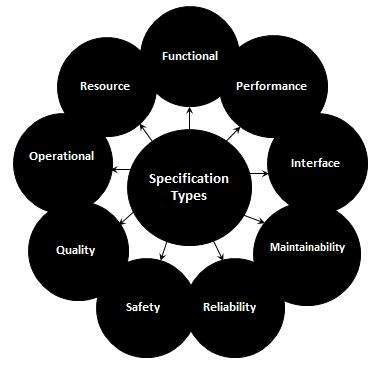
\includegraphics[scale=0.75]{components/4/pics/frs_req.jpg}
  \caption{Applied on N2Sky  Requirement Specification Quialities}
  \label{fig:frs_req}
\end{center}
\end{figure}



\subsection{User Roles}\label{User Roles}

In order to make the N2Sky user interface understandable for arbitrary users as well as professional for advances users, it was decided to separate the user roles. Every user role has own way of interaction with the application:

Every user has some specific area within he works. For example just registered user does not need to know the current environment monitoring information. These restrictions were motivation to create some user roles in order to restrict of grand some functionality of N2Sky as it shown on ``Fig.~\ref{fig:userroles}''.

\begin{figure}[htbp]
\begin{center}
  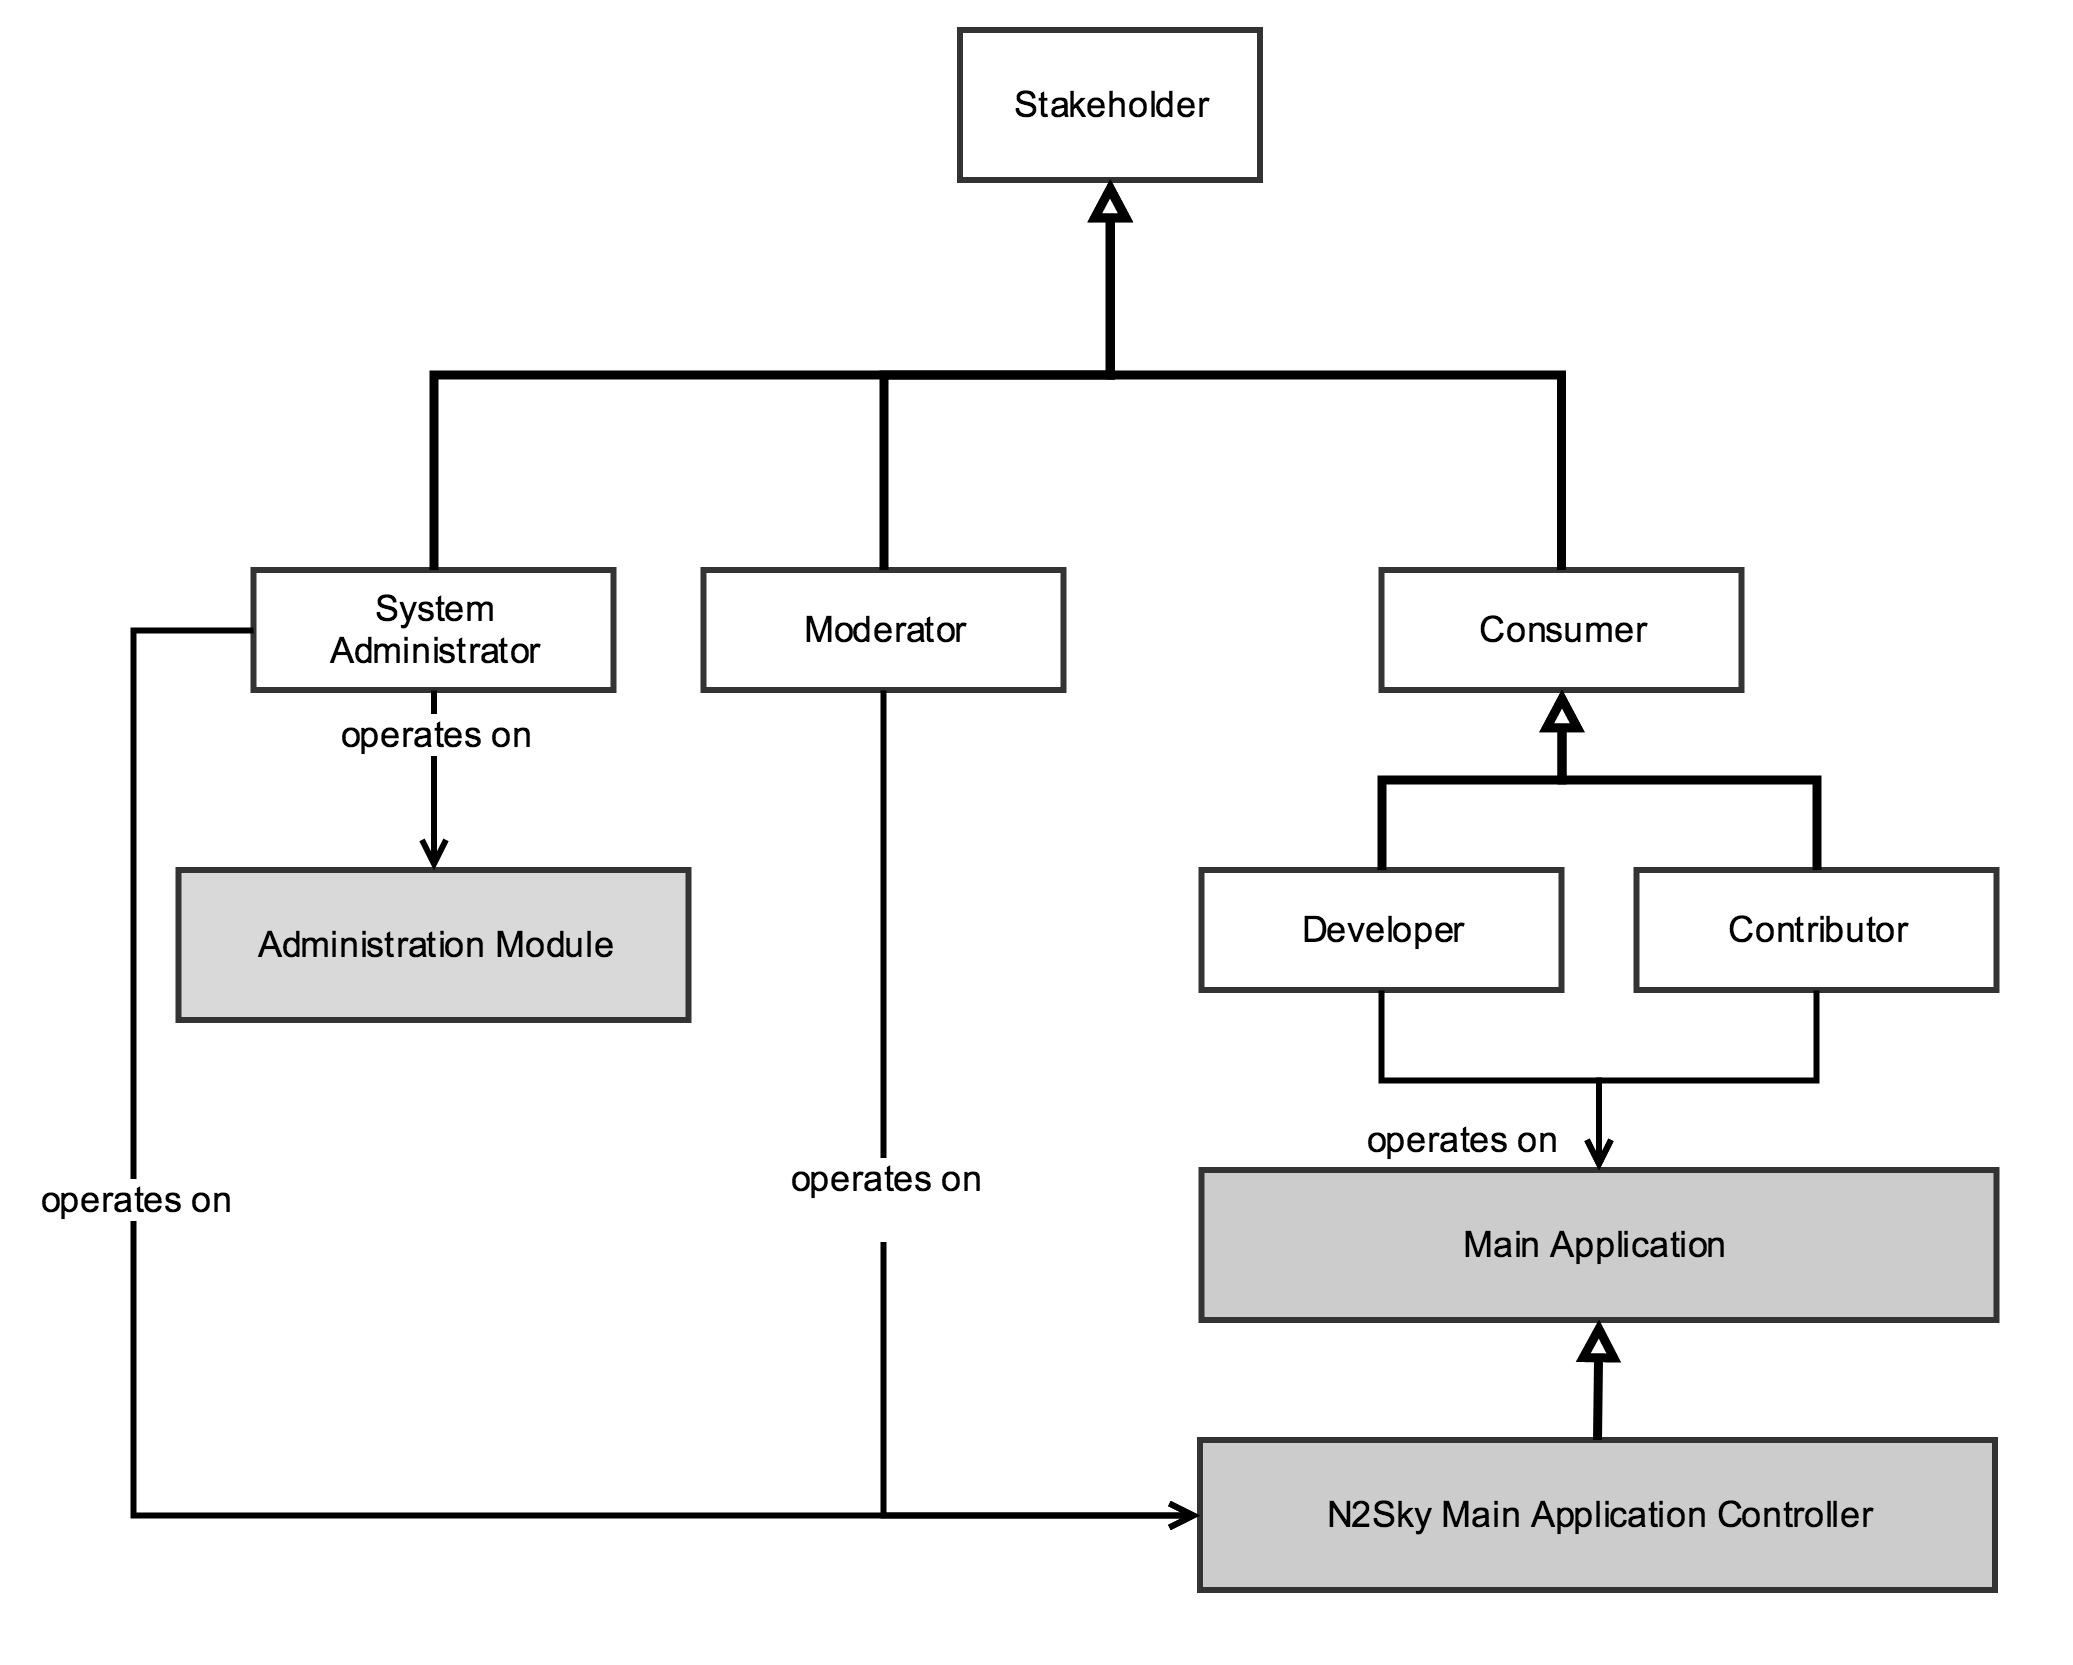
\includegraphics[width=\linewidth]{components/4/users.png}
  \caption{User roles hierarchy and modules where they operating on (marked grey)}
  \label{fig:userroles}
\end{center}
\end{figure}

\begin{description}
\item[Contributor.]   The Contributor is an arbitrary user. Such a user has no necessity in having deep knowledge of the neural network field or know any programming language. The main goal of arbitrary user is to study neural networks within N2Sky. The contributor has access only to his own dashboard and public available resources on the main application module. He can perform semantic search for available neural network paradigms and use them. He can also train running neural network instances and test them. This user can share his trained neural network by making it public. 
\item[Consumer.] The Consumer is an arbitrary user, except he is not creating but using already existing neural networks and trained models. His main purpose is to evaluate trained models or execute training against existing neural networks. This kind of user does not have to use his own training data, he just wants to see the behaviour of neural networks. The Consumer can be converted to Contributor user if he has enough knowledge for it. 
\item[Developer.] The Developer is an expert user, which has enough knowledge and experience to create his own neural network. This user can create neural network paradigms using the ViNNSL schema and publish them on N2Sky. This user can deploy neural networks on the N2Sky environment as well as on his own environment by providing training and testing endpoints. The goal of the developer is the study how his networks will behave with different network structures, input parameters and training data that is provided by other users.
\item[System Administrator.] System Administrator is a user who has a full access to application including environment management, monitoring and alerting features. Administrator can manage Openstack and Cloudify instances. He also can shadow any N2Sky user to observe the application from shadowed user perspective. Administrator has access to all dashboards in every module.
\item[Moderator.] Is a user with a granted permissions. This user can moderate Main Application Module namely neural network instances and  trained models from other users. The Moderator does not have access to Administration Module and can not be converted to System Administrator user role.
\end{description}

\subsection{User Main Functions}\label{User Permissions}

In more detailed overview of user roles it is possible to define permission and main functions.
Permissions describes users allowed page view. If user has access to particular page view the main user function can be defined. 
The main user function characterise allowed behaviour on particular page view. 

As it was mentioned in previous chapter,  N2Sky is an modular application. Permissions and main functions of Administration Module and N2Sky Main Application Controller, which is a part of Main Application Modules, described in Table \ref{table:admin}.

\begin{table}[]
\resizebox{\textwidth}{!}{%
\begin{tabular}{|l|c|c|c|c|c|c|c|c|}
\hline
\multicolumn{1}{|c|}{User Role} & \multicolumn{2}{c|}{\textbf{Administration Module}}          & \multicolumn{2}{c|}{\textbf{N2Sky Main Application Controller}}      \\ \hline
\multicolumn{1}{|c|}{\textbf{}} & \textbf{OpenStack Management} & \textbf{Cloudify Management} & \textbf{Neural Networks Management} & \textbf{Trained Models Management} \\ \hline
System Administrator            & \textbf{+}                    & \textbf{+}                   & \textbf{+}                          & \textbf{+}                            \\ \hline
Moderator                       & \textbf{-}                    & \textbf{-}                   & \textbf{+}                          & \textbf{+}              \\ \hline
Consumer                        & \textbf{-}                    & \textbf{-}                   & \textbf{-}                          & \textbf{-}                            \\ \hline
Developer                       & \textbf{-}                    & \textbf{-}                   & \textbf{-}                          & \textbf{-}                               \\ \hline
Contributor                     & \textbf{-}                    & \textbf{-}                   & \textbf{-}                          & \textbf{-}                    \\ \hline
\end{tabular}%
}
\caption{User Roles main functions considering "Administration Module" and "N2Sky Main Application Controller". 
"+" for allowed, "-" for disallowed}
\label{table:admin}
\end{table}

System Administrator has permissions to all components. Moderator has access only to N2Sky Main Application Controller. Since both of this user roles extending Contributor user role, the permissions for main application module are also granted.

Consumer, Developer and Contributor user roles have no access to any administration parts of N2Sky. This users do not have any main function in this area, but they can operate N2Sky Main Application Module as it shown on Table \ref{table:main}.

\begin{table}[]
\resizebox{\textwidth}{!}{%
\begin{tabular}{|l|c|c|c|c|}
\hline
\multicolumn{1}{|c|}{User Role} & \multicolumn{4}{c|}{\textbf{N2Sky Main Application Module}}                                                                                    \\ \hline
\multicolumn{1}{|c|}{\textbf{}} & \textbf{Paradigm Creation} & \textbf{Neural Networks Creation} & \textbf{Neural Network Training} & \textbf{Training Models Evalutaion} \\ \hline
System Administrator            & \textbf{-}                 & \textbf{-}                        & \textbf{-}                       & \textbf{-}                          \\ \hline
Moderator                       & \textbf{-}                 & \textbf{-}                        & \textbf{-}                       & \textbf{-}                          \\ \hline
Consumer                        & \textbf{-}                 & \textbf{-}                        & \textbf{+}                       & \textbf{+}                          \\ \hline
Developer                       & \textbf{+}                 & \textbf{+}                        & \textbf{+}                       & \textbf{+}                          \\ \hline
Contributor                     & \textbf{-}                 & \textbf{+}                        & \textbf{+}                       & \textbf{+}                          \\ \hline
\end{tabular}%
}
\caption{User Roles main functions considering "N2Sky Main Application Module". 
"+" for allowed, "-" for disallowed}
\label{table:main}
\end{table}

As it was mentioned before System Administrator as well as Moderator has access to N2Sky Main Application Module, but they do not have a main function there. On the other hand all user roles, which are extending consumer can contribute in a N2Sky Main Application Module, except Consumer itself. Consumer has access to all page views on this module, but he has another purpose. 

\subsection{N2Sky Main Application Module Components}\label{N2Sky Components}
\subsubsection{Affected user groups}\label{Affected user groups 2}
\subsubsection{N2Sky Dashboard}\label{N2Sky Dashboard}
\subsubsection{Neural Networks Repository}\label{Neural Networks Repository}
\subsubsection{Models Repository}\label{Models Repository}

\subsection{Requirements specifications for Administration Module}\label{Administration components}

\subsubsection{General Definition}\label{General Definition AMC}

Administration Module Component (AMC) is an application, which is responsible for managing OpenStack and Cloudify. It has embedded Monitoring System and Alert Management System. AMC is integrated in N2Sky cloud platform in order to support N2Sky environment and services. This component is implementing Platform as a service approach, hence it can be installed on any cloud server. 

\subsubsection{Affected users}\label{Affected users}

The users, who has full knowledge about domain with corespondent permissions or domain owner can has an access to AMC.

In N2Sky only System Administrator has a proper main function in order to manage AMC.
Following functions are available for System Administrator:
\begin{itemize}
\item Mange own dashboard view
\item Control OpenStack Dashboard and its services
\item Control Cloudify Dashboard and its services
\item Manage monitoring charts
\item Manage alerts and alerting rules
\item Managet OpenStack instances (servers)
\item Has an access to dashboards of other users
\end{itemize}



\subsubsection{FRS for Administration Dashboard}\label{Administration Dashboard}

Administration Dashboard represents overview of administration tools and important metrics, which is desplayed in ``Fig.~\ref{fig:admin_dashboard}''. 

\begin{figure}[htbp]
\begin{center}
  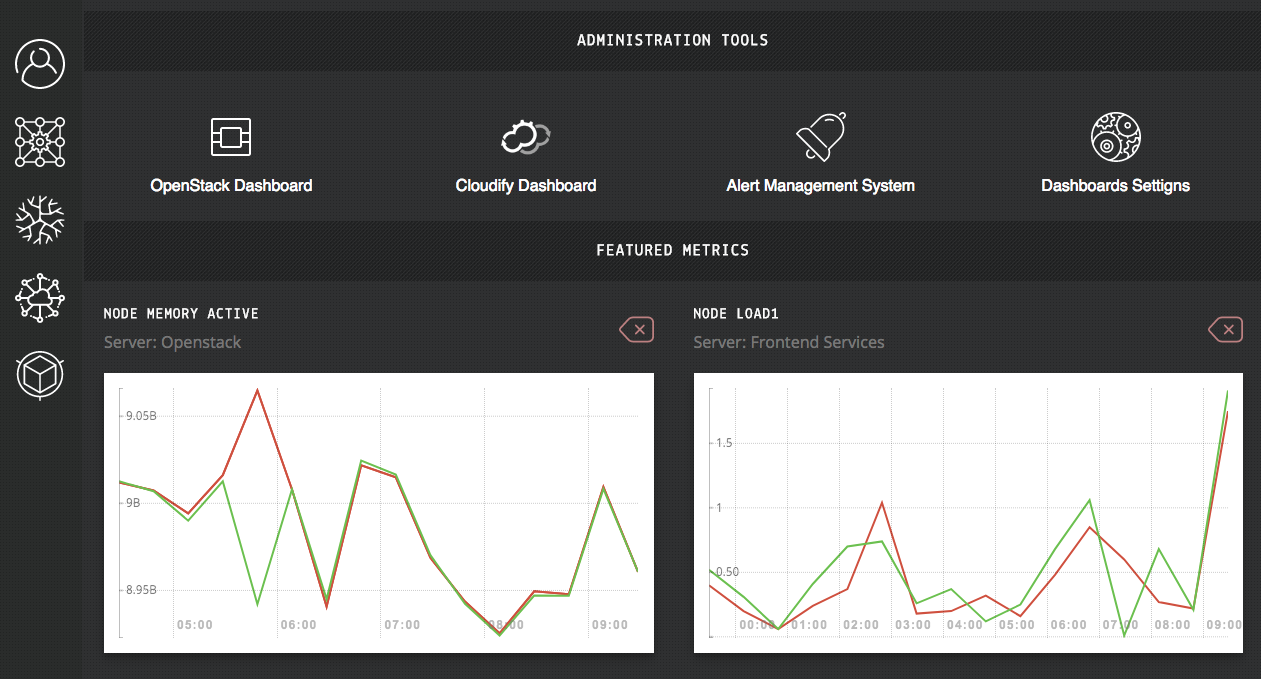
\includegraphics[width=\linewidth]{components/4/pics/admin_dashboard.png}
  \caption{N2Sky Administration Dashboard.}
  \label{fig:admin_dashboard}
\end{center}
\end{figure}

After System Administrator login into system he will be automaticly redirected to Administration Dashboard. By default url link is:
\begin{lstlisting}
		<host>/cloud
\end{lstlisting}

Administration tools has to be in focus of main dashboard view as it shown in ``Fig.~\ref{fig:admin_tools}''. The collection of elements has to be under the title bar element, which has name "ADMINISTRATION TOOLS". Every element of administration tool has to contain icon in SVG \cite{Cagle2005} format and caption under it. Following administration tools has to be represented: 
\begin{itemize}
\item OpenStack Dashboard. Link to view: 
\begin{lstlisting}
		<host>/openstack
\end{lstlisting}
\item Cloudify Dashboard. Link to view: 
\begin{lstlisting}
		<host>/cloudify
\end{lstlisting}
\item Alert Management System. Link to view: 
\begin{lstlisting}
		<host>/alert
\end{lstlisting}
\item Dashboards Settings. Modal popup window without redirection
\end{itemize}

\begin{figure}[htbp]
\begin{center}
  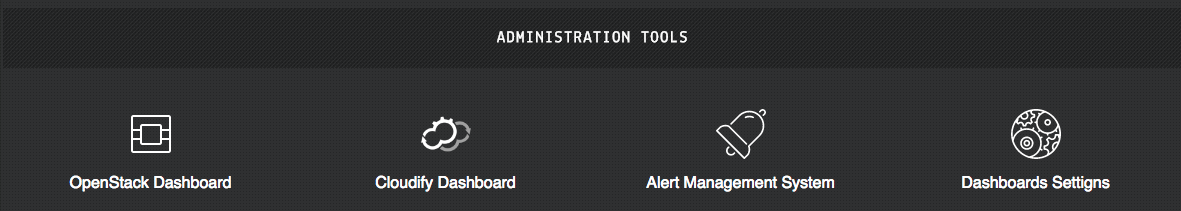
\includegraphics[width=\linewidth]{components/4/pics/admin_tools.png}
  \caption{N2Sky Administration Dashboard. Administration tools component.}
  \label{fig:admin_tools}
\end{center}
\end{figure}

Next to administration tools the monitoring charts are showing. The title of this block is "FEATURED METRICS", which is the tile of bar upon the metrics.
Every chart is a grid item element, the grit itself has to contain maximum two grit items in one row as it shown in ``Fig.~\ref{fig:featured_metrics}''. 
 
\begin{figure}[htbp]
\begin{center}
  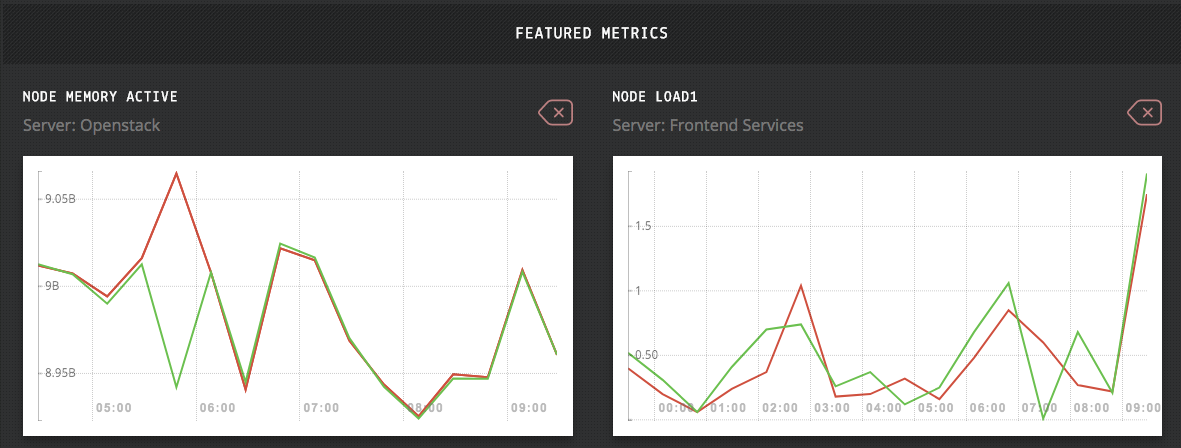
\includegraphics[width=\linewidth]{components/4/pics/featured_metrics.png}
  \caption{N2Sky Administration Dashboard. Featured Metrics component.}
  \label{fig:featured_metrics}
\end{center}
\end{figure}
 
 
The user decides by him self which monitoring charts will be shown. The configuration is located in "Dashboard Settings" administration tool element. More details about creation of monitoring charts is located in \autoref{Monitoring System}. 


\subsection{FRS for Openstack Dashboard}\label{OpenStack Dashboard}

OpenStack Dashboard is the dashboard for managing OpenStack and its services and monitoring OpenStack and its instances. It looks similar to Administration Dashboard, except it is only OpenStack oriented and there is not additional tools as it shown in ``Fig.~\ref{fig:openstack_dashboard}''. 

\begin{figure}[htbp]
\begin{center}
  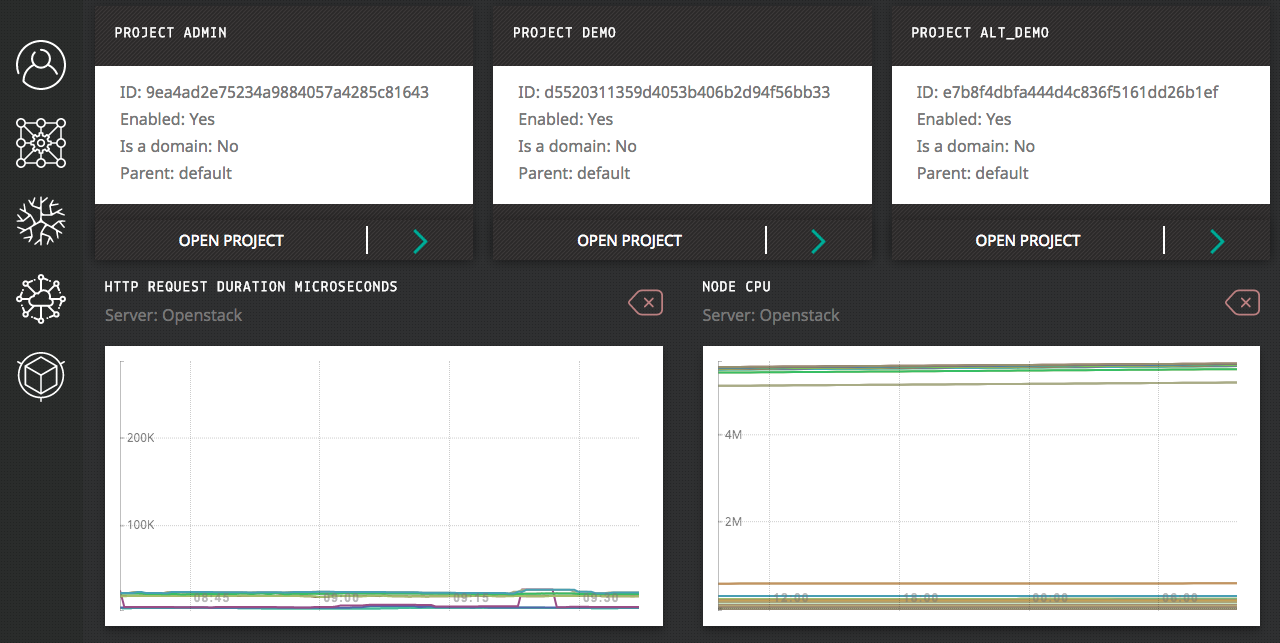
\includegraphics[width=\linewidth]{components/4/pics/openstack_dashboard.png}
  \caption{N2Sky OpenStack Dashboard.}
  \label{fig:openstack_dashboard}
\end{center}
\end{figure}
 

This dashboard contains two blocks:

\begin{description}
\item[Project grid.] This block contains projects, which are available on OpenStack as it shown in ``Fig.~\ref{fig:openstack_dashboard_projects}''.

\begin{figure}[htbp]
\begin{center}
  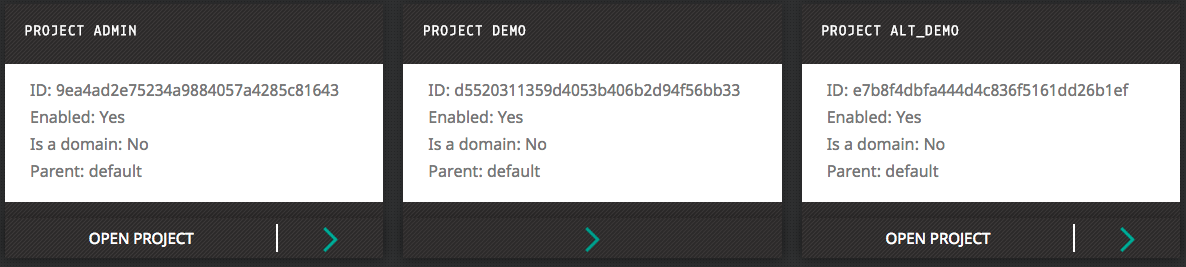
\includegraphics[width=\linewidth]{components/4/pics/openstack_dashboard_projects.png}
  \caption{N2Sky OpenStack Dashboard. Projects grid}
  \label{fig:openstack_dashboard_projects}
\end{center}
\end{figure}

Every grid item represents brief overview about OpenStack Project:

\begin{itemize}
\item Name of the project, which is header of grid item.
\item ID of project.
\item Enabled, which stays if available (value YES) or not available (value NO).
\item Is a domain, also contains simple yes or no values.
\item Parent, which says if there any parent project which is current project linked.
\item Button "Open Project", which redirects to project details.
\end{itemize}

\item[Monitoring Grid.] Similar to Administration Dashboard monitoring grid can be customised by users. Detail information about customisation is written in \autoref{Monitoring System}. 

\end{description}

After redirecting to project details the user will see information about specific project. Redirection should hast following URL path: 
\begin{lstlisting}
		<host>/openstack/project/<id>
\end{lstlisting}

Where <id> is OpenStack project ID.

\subsubsection{OpenStack Nova Service}\label{OpenStack Nova Service}

Nova is a compute service of OpenStack. I gives overview and managing of all existing virtual machine (servers or isntances) \cite{Markelov2016}. 

Following tools for using compute service:
\begin{itemize}
\item Horizon. Web UI for managing OpenStack projects. It is not used in N2Sky system since N2Sky Web UI has its own interface for managing the OpenStack instances.
\item OpenStack Client, which is includes commands for nova as well as for OpenStack projects.
\item Nova Client, which can be use like OpenStack Client, but N2Sky does not use it since OpenStack Client can provide all needed commands for nova service. 
\end{itemize}


OpenStack project view has detailed description about server and its instances as it shown in ``Fig.~\ref{fig:openstack_dashboard_projects}''. 

\begin{figure}[htbp]
\begin{center}
  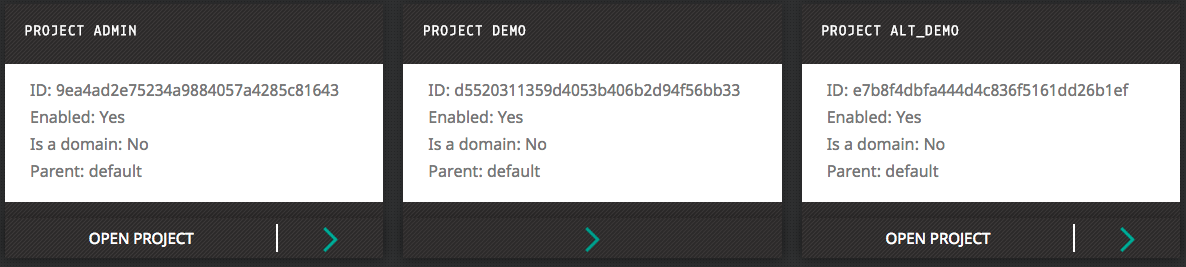
\includegraphics[width=\linewidth]{components/4/pics/openstack_dashboard_projects.png}
  \caption{N2Sky OpenStack Dashboard. Project view}
  \label{fig:openstack_dashboard_projects}
\end{center}
\end{figure}

This view contains following components:
\begin{description}
\item[Navigation Bar.] Navigation over OpenStack Services namely:
\begin{itemize}
\item NOVA
\item NEUTRON
\item IMAGES
\item VITRAGE
\end{itemize}
 
 \item[Servers.] Servers item grid is located on the left size of the screen and has an collection of servers (OpenStack instances) as it shown in ``Fig.~\ref{fig:openstack_servers}''. 
 
 \begin{figure}[htbp]
\begin{center}
  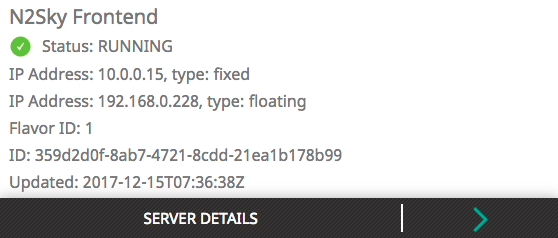
\includegraphics[scale=0.6]{components/4/pics/openstack_servers.png}
  \caption{N2Sky OpenStack Dashboard. Server overview}
  \label{fig:openstack_servers}
\end{center}
\end{figure}

The server overview grid contains following elements:
\begin{itemize}
\item Server name 
\item Status, which can be: 
\begin{itemize}
\item RUNNING - instance is running and available. 
\item SHUTOFF - instance is manually or by schedular shuted down. 
\item ERROR - an error occur during spawning an instance or instance went down during run.
\end{itemize}
\item IP Address fixed. The IP Address of instance inside OpenStack Cloud.
\item IP Address floating. Assigned to instance IP address. Through this IP address an external access to instance is possible. 
\item Flavor ID. Reference on OpenStack flavor, which is located on the right side of OpenStack project view.
\item ID of server (OpenStack instance).
\item Updated is timestamp when instance was last time modified. 
\end{itemize}
\item[Flavors.] A flavor is define an environment configuration. In the project details view there are list of flavors. On click on particular flavor of this list, the flavor details will appear as it shown in ``Fig.~\ref{fig:openstack_flavors}''.

 \begin{figure}[htbp]
\begin{center}
  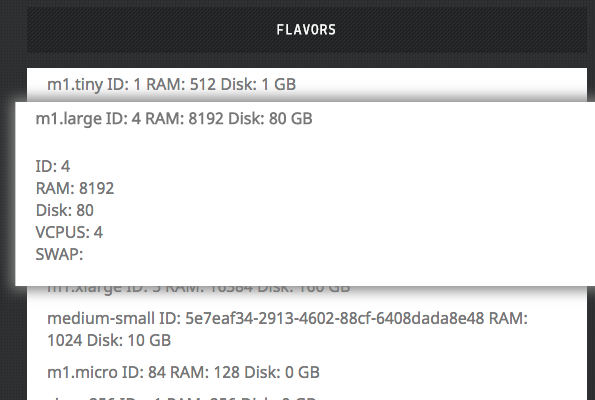
\includegraphics[scale=0.6]{components/4/pics/openstack_flavors.png}
  \caption{N2Sky OpenStack Dashboard. Flavors}
  \label{fig:openstack_flavors}
\end{center}
\end{figure}

Following elements are displayed: 
\begin{itemize}
\item Type of flavor, which is defined by OpenStack.
\item ID of flavor. OpenStack instances have a reference on particular flavor ID
\item RAM. Amount of available memory of particular flavor. 
\item Disk space in GB, which is available for particular flavor. 
\item VCPUS. About of CPUs which will be available. 
\item SWAP in GB, which is set for particular flavor.
\end{itemize}

\end{description}

When user choose some server (instance), he will be redirected to server details view as it shown in ``Fig.~\ref{fig:openstack_server_details}''.

 \begin{figure}[htbp]
\begin{center}
  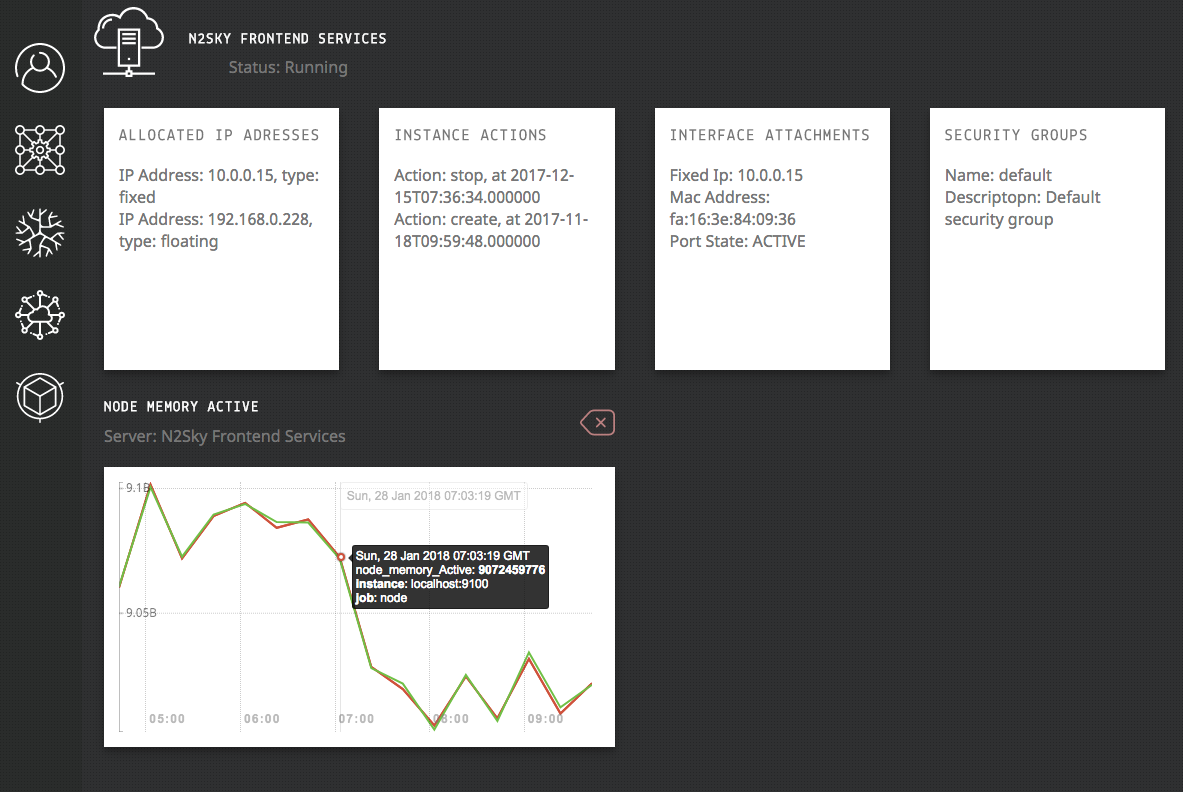
\includegraphics[width=\linewidth]{components/4/pics/openstack_server_details.png}
  \caption{N2Sky OpenStack Dashboard. Server details view.}
  \label{fig:openstack_server_details}
\end{center}
\end{figure}

\subsubsection{OpenStack Neutron Service}\label{OpenStack Neutron Service}

Neutron is an OpenStack networking service, which provides "network connectivity as a service". Neutron is fully integrated in OpenStack UI, which allows to manage networking directly from there. The networking service is based on quantum architecture, where API clients communicate with virtual switches through Quantum APU and Quantum plugin \cite{neutron}. This service implements Neutron API, which is used by N2Sky Web UI. 

Neutron Service is integrated in N2Sky and represents overview of networks, subnet pools and services providers as it shown in ``Fig.~\ref{fig:openstack_neutron}''.

\begin{figure}[htbp]
\begin{center}
  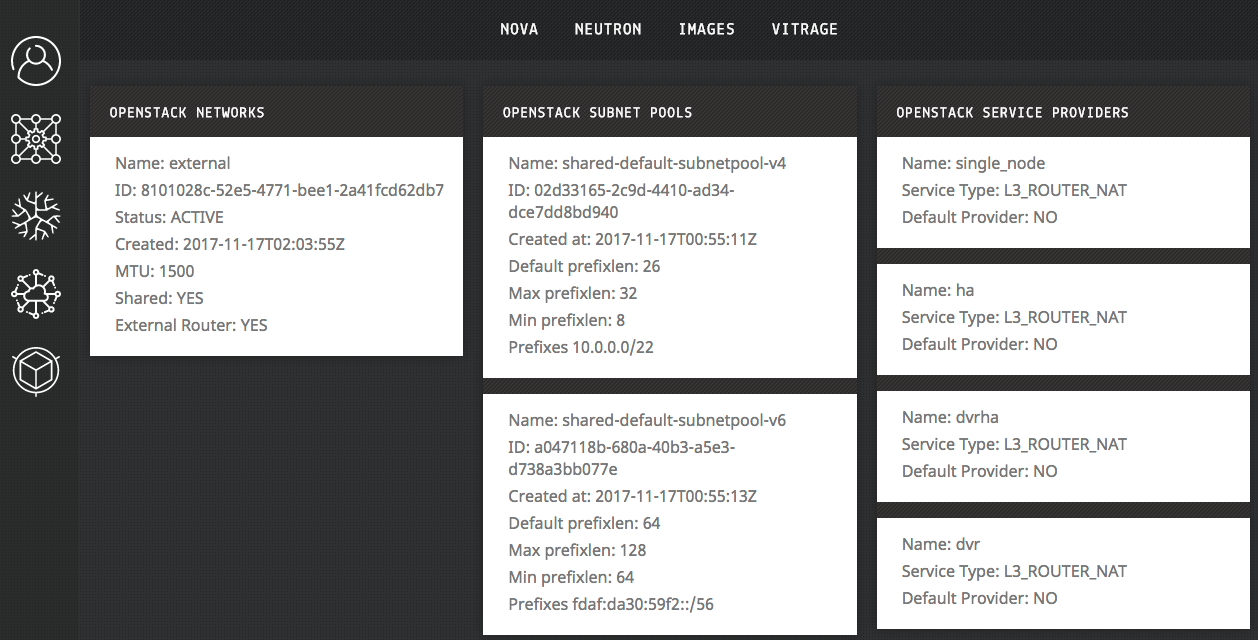
\includegraphics[width=\linewidth]{components/4/pics/openstack_neutron.png}
  \caption{N2Sky OpenStack Dashboard. Neutron Service View}
  \label{fig:openstack_neutron}
\end{center}
\end{figure}

The server details view contains following components:
\begin{description}
\item[Header.] Header of this view  contains the name of the server, icon and status, which can be "Running" if instance is available and running on OpenStack environment, "Shutdown" if instance is available but nut running and "Error" in case if an error occurred. 
\item[Instance information grid]. Following grid represents summary information about server (instance) and consist of following grid items:
\begin{itemize}
\item Allocated IP Addresses is a list of assigned to instance IP addresses. Every IP address has a type either "fixed" or "floating".
\item Instance actions is a list of all action and events, which happened with particular instance. Log information contains action type and timestamp of action.
\item Interface attachments, which contains fixed IP address, mac address add port state ("ACTIVE" or "INACTIVE") of the instance.
\item Security groups is a list of security groups which contains the name and description of security group . 
\end{itemize}
\item[Monitoring.] The grid of monitoring charts of particular server. Can be removed directly from the view or added via navigation menu or Administration Dashboard.
\end{description}


The grid represents following componsnts besides navigation bar: 
\begin{description}
\item[OpenStack Networks.]  The list of available networks on OpenStack cloud. Every network contains following information:
\begin{enumerate}
\item Name of the network
\item ID of the network
\item Status, which can be "ACTIVE" network is available and "INACTIVE" is it not available or an error occurred. 
\item Created is timestamp of creation of the network
\item MTU (Network Service Uses), which are based on physical network in order to calculate MTU of virtual network components. 
\item Shared. "YES" for shared access and "NO" for not shared accordantly. 
\item External router. "YES" for external router is attached and "NO" for not attached accordantly. 
\end{enumerate}
\item[OpenStack Subnet Pools.] This service provides information about available subnetworks and includes following information on N2Sky application:
\begin{enumerate}
\item Name of the subnetwork
\item ID of the subnetwork
\item Created at is the timestamp of subnetwork creation
\item Default number prefixlen
\item Max number of prefixlen
\item Min number of prefixlen
\item Prefixlen, which represents a pool profix
\end{enumerate}
\item[OpenStack Service Providers.] The list of created and available service providers with customised configuration, which contains:
\begin{enumerate}
\item Name of service provider
\item Service type
\item Default provider. "YES" if exist, "NO" if not accordantly.  
\end{enumerate}

\end{description}


\subsubsection{OpenStack Images Service}\label{OpenStack Images Service}

In OpenStack is possible to upload customised images of the Virtual Machine to the provider. N2Sky uses Images Service only for representation of images information. It also possible to download image, but it is not possible to upload customised image due expensive process, because of the size of images. It is possible to use template provider with pre-configured virtual machine \cite{images}. 


\begin{figure}[htbp]
\begin{center}
  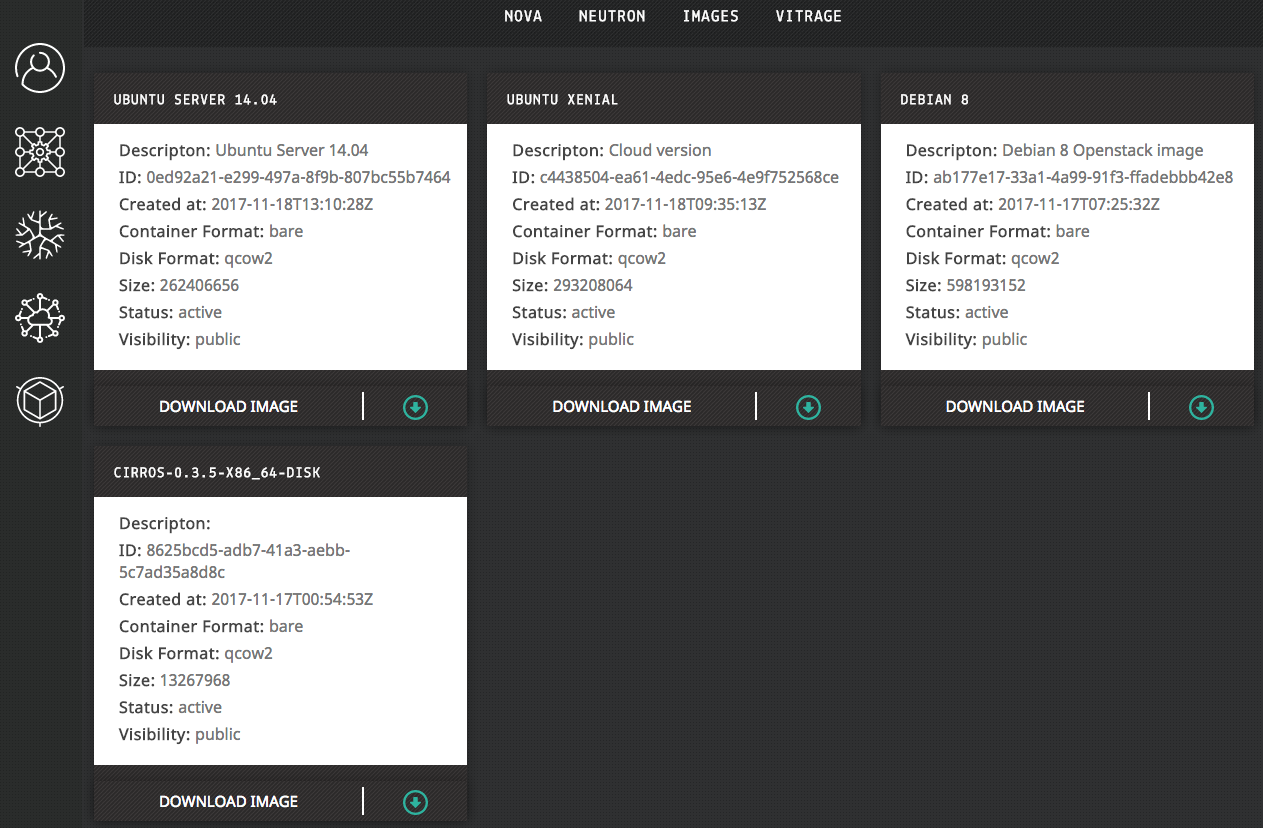
\includegraphics[width=\linewidth]{components/4/pics/openstack_images.png}
  \caption{N2Sky OpenStack Dashboard. Images Service View}
  \label{fig:openstack_images}
\end{center}
\end{figure}

The Image Service view, which shown in ``Fig.~\ref{fig:openstack_images}'' is representing a grid of available images. Every grid item contains following information: 
\begin{enumerate}
\item Name of the image
\item Description of the image
\item ID of the image
\item Created at, which represents the timestamp of the creation date of the image
\item Container format
\item Disk format namely format of the image (qcow2 is a typical format for OpenStack instance)
\item Size of the image in bytes
\item Status of the image. Active if image is successfully upload and ready to use, inactive if it not
\item Visibility. Public for everyone or group name for particular group of OpenStack users
\item Download image button, which create one more thread an initialise downloading procedure
\end{enumerate}

There are custom OpenStack image templates and configuration created for N2Sky system. Every image has to contain following configuration:
\begin{itemize}
\item Preinstalled Docker CLI
\item N2Sky Monitoring System instance
\item N2Sky Alert Management System rules configuration
\end{itemize}

N2Sky templates and configuration has to support following operating systems:
\begin{itemize}
\item Ubuntu 14.04 / 16.04 
\item Debian 8
\item Centos
\end{itemize}



\subsubsection{OpenStack Vitrage Service}\label{OpenStack Vitrage Service}

Vitrage is the OpenStack RCA (Root Cause Analysis) service. Is a build in monitoring system, which helps to analyse and organise OpenStack alarms and events \cite{wiki:vitrage}. In N2Sky platform Vitrage service is used only for representation of  templates and resources, because N2Sky has its own Monitoring System, which can be propagate in all OpenStack instances.  

\begin{figure}[htbp]
\begin{center}
  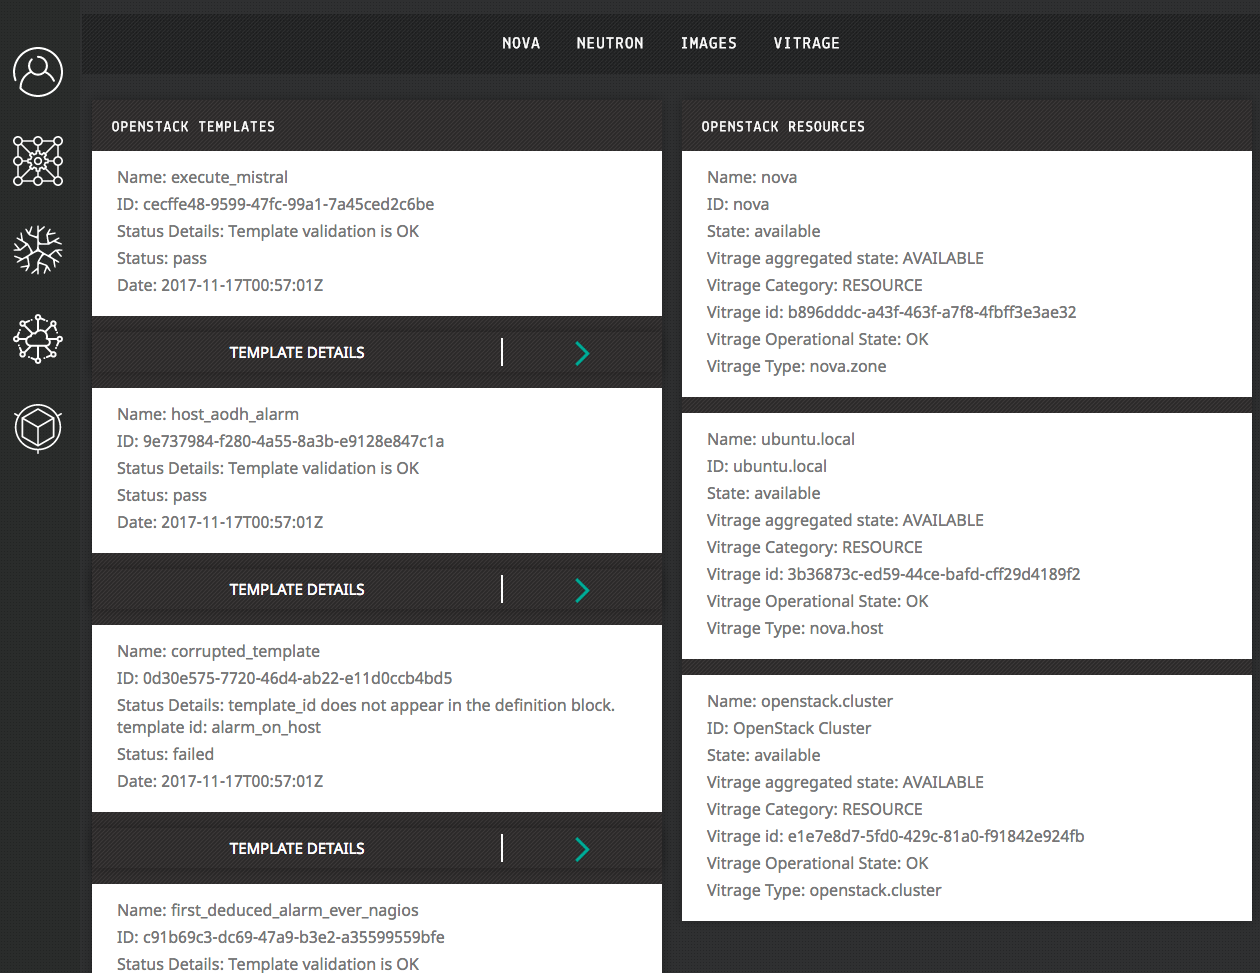
\includegraphics[width=\linewidth]{components/4/pics/opentack_vitrage.png}
  \caption{N2Sky OpenStack Dashboard. Vitrage Service View}
  \label{fig:opentack_vitrage}
\end{center}
\end{figure}

Two column grid view which is shown in ``Fig.~\ref{fig:opentack_vitrage}'' represents following grid items:

\begin{description}
\item[OpenStack Templates.]  List of OpenStack templates with following data:
\begin{enumerate}
\item Name of the template
\item ID of the template
\item Status Details, which shows if the template validated 
\item Date, which shows timestamp of template creation 
\item Template details button, which redirect in detailed information about chosen template
\end{enumerate}

\item[OpenStack Resources.] List of available OpenStack resources, which contains following data:
\begin{enumerate}
\item Name of the resource
\item ID of the resource
\item State of the resource, can be available or not available
\item Vitrage aggregated state, can be available or not available
\item Vitrage Category, can be resource, alarm or other customised catefory
\item Vitrage ID
\item Vitrage Operational State
\item Vitrage Type
\end{enumerate}
\end{description}

\begin{figure}[htbp]
\begin{center}
  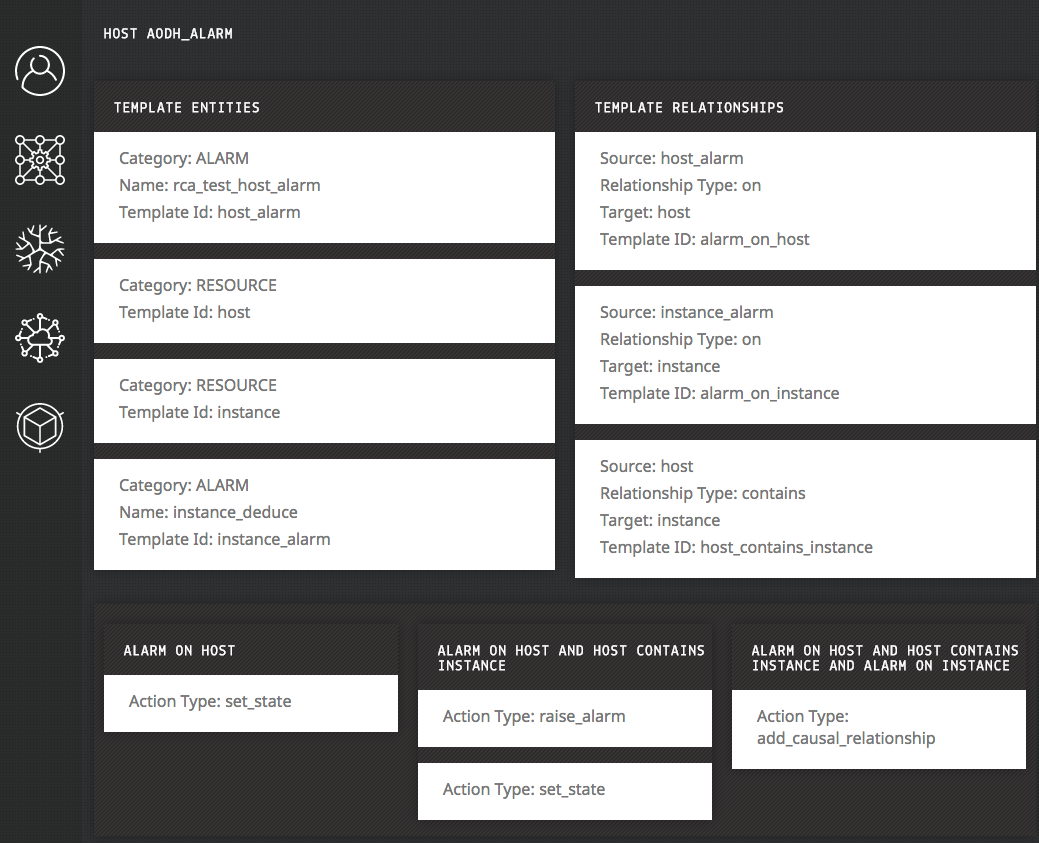
\includegraphics[width=\linewidth]{components/4/pics/openstack_template.png}
  \caption{N2Sky OpenStack Dashboard. Template Details View}
  \label{fig:openstack_template}
\end{center}
\end{figure}

When user click on template details button he will be redirected on particular Vitrage template as it shown in ``Fig.~\ref{fig:openstack_template}''. From here user can observe following information:
\begin{description}
\item[Template Entities]. List of entities like alarm or resource. This grid item contains following data
\begin{enumerate}
\item Template ID (mandatory)
\item Name of the template (optional)
\item Template category (optional)
\end{enumerate}
\item[Template Relationships]. List of relationships between templates, which reference from source to target.
\begin{enumerate}
\item Source entity
\item Target entity
\item Relationship type
\item Template ID
\end{enumerate}
\item[Alarm On Host.] The action type of the alarm
\item[Alarm on host and host contains instance.] Optional item, visible only of host contains instance.
\item[Alarm on host and host contains instance and alarm on instance.] Optional item, visible only of host contains instance and alarm on instance.

\end{description}



\subsection{FRS for Cloudify Dashboard}\label{Cloudify Dashboard}

\hl{TODO ????}

\subsection{Dashboard Settings}\label{Dashboard Settings}
As it was mentioned before in Administration Dashboard chapter \autoref{Administration Dashboard}, the dashboard has the administration tools. One of this tools is Dashboard Settings tool. When user click on this tool the modal popup window will open and available configuration options will appear as it shown in ``Fig.~\ref{fig:openstack_template}''.

\begin{figure}[htbp]
\begin{center}
  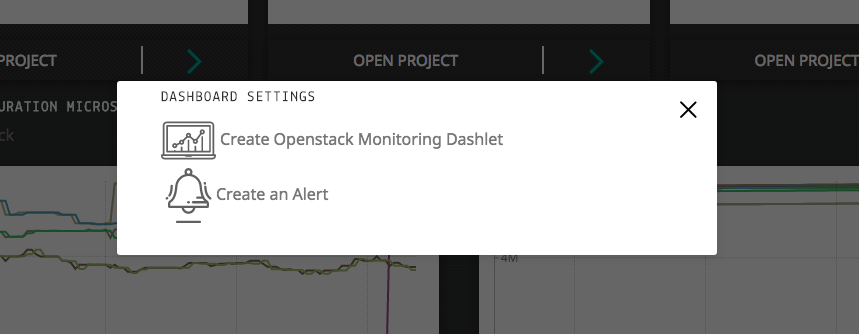
\includegraphics[width=\linewidth]{components/4/pics/dashboard_settings.png}
  \caption{N2Sky Administration Dashboard. Dashboard Settings}
  \label{fig:dashboard_settings}
\end{center}
\end{figure}

Another one possibility to initiate settings popup is to open it from main navigation menu, which is available across entire application on the left screen of the page view. 

Dashboard Settings popup contains two setting for now:
\begin{itemize}
\item Create OpenStack Monitoring Dashlet, which create one more modal popup upon existing and initialise creation monitoring chart, which is described in chapter "Monitoring System" in \autoref{Monitoring System}.
\item Create an Alert, which also create one more modal popup upon existing and initialise creation alerting rule, which is described in chapter "Alert System" in \autoref{Alerting System}.
\end{itemize}

The popup will be automatically closed only after action performed, if action is not performed user can leave the popup manually.



\subsection{Monitoring System}\label{Monitoring System}

When Administration Dashboard in general shows overview of the OpenStack and Cloudify, the monitoring system goes through every dashboard an apply monitoring chars on user request. There are two main parts, which has to be mentioned in FRS: displaying of monitoring charts and management of metrics.
 
\subsubsection{Monitoring charts creation}\label{Monitoring charts creation}

After user initialise creation of monitoring metrics at it was described in \autoref{Dashboard Settings} "Dashboard Settings", a new modal window will be opened as it shown in ``Fig.~\ref{fig:create_monitoring}''.

\begin{figure}[htbp]
\begin{center}
  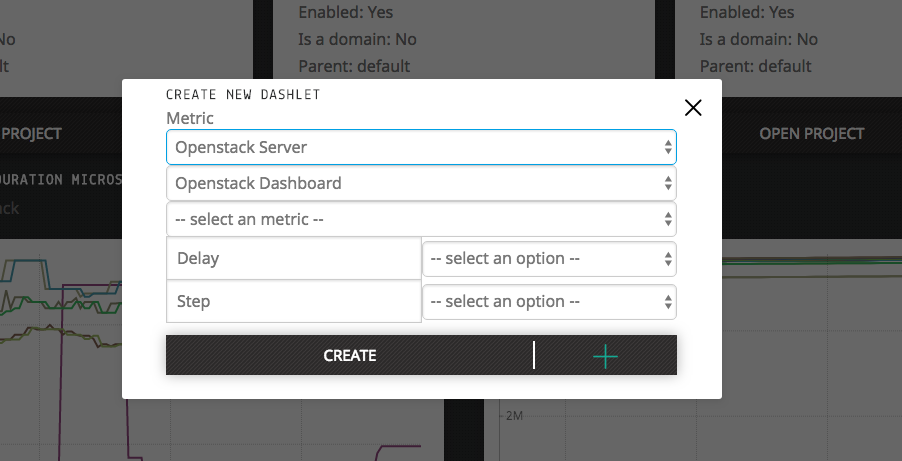
\includegraphics[width=\linewidth]{components/4/pics/create_monitoring.png}
  \caption{N2Sky Administration Dashboard. Monitoring charts creation modal popup}
  \label{fig:create_monitoring}
\end{center}
\end{figure}

The popup window has following elements:

\begin{enumerate}
\item "CREATE NEW DASHLET" title of the popup
\item Combobox with servers, where monitoring system instance is installed. User can choose all available instances, even if they are not running currently. It is also possible to choose OpenStack cloud server itself, because monitoring system instance is preinstalled there.
\item Combobox with views.  User can choose where combobox will be added. There are few places where chart can be displayed:
\begin{enumerate}
\item Administration Dashboard
\item OpenStack Dashboard
\item Cloudify Dashboard
\item Servers (OpenStack instances) View. 
\end{enumerate}
\item Combobox with metrics. Normally it is more then hundred of available metrics. It is important to mention that every operating system has different naming of metrics.
\item Delay input. This input shows the delayed time of metric.
\item Step input. This input shows the line chart step of chosen metric
\item Timing combobox. This combobox contains following time options:
\begin{enumerate}
\item seconds
\item minutes
\item hours
\item days
\item weeks
\end{enumerate}
\item Create button, which trigger metrics creation. The view will be reloaded and monitoring chart will appear on this view.
\end{enumerate}

After adding a new monitoring chart, the view will be reloaded and the chart will appear on the view. 

\subsubsection{Monitoring charts representation}\label{Monitoring chart representation}

Every monitoring chart is a grid item of two column responsive grid as it shown in ``Fig.~\ref{fig:moniroting_representation}'' 

\begin{figure}[htbp]
\begin{center}
  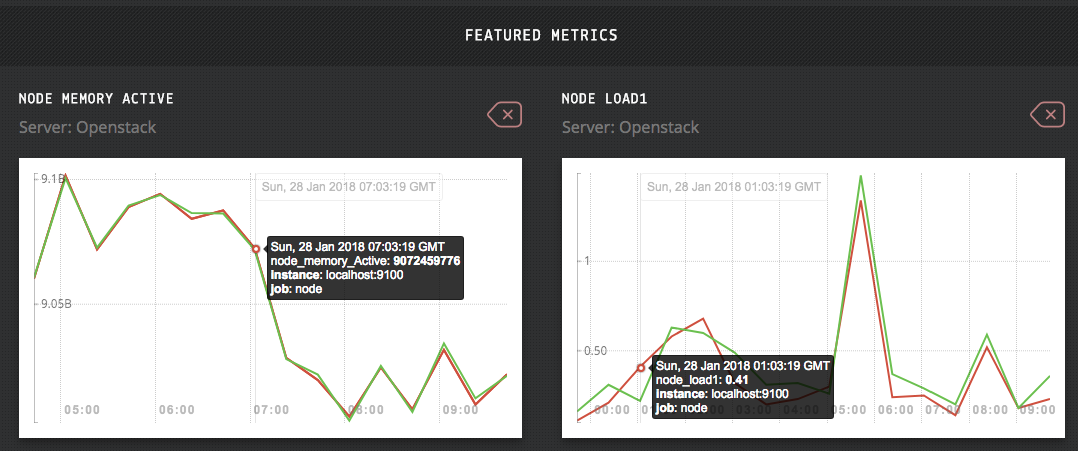
\includegraphics[width=\linewidth]{components/4/pics/moniroting_representation.png}
  \caption{N2Sky Administration Dashboard. Monitoring charts representation}
  \label{fig:moniroting_representation}
\end{center}
\end{figure}

The grid hast to be responsive in order to support mobile devices. When mobile device is detected the grid should has only one column and grid items has ti be aligned vertically. 

The header of monitoring chart has to contains the name of the metrics and the server (instance) from where this metrics comes.

Every monitoring chart has at list one line graph with a random colour. If there are few line graphs in the chart, then lines has to have a different colour. A chart contains on x-Axis the timestamp and on y-Axis the velocity.  The timestamp in line graph has its own toolkit with additional information about the chart and contains following data:

\begin{itemize}
\item Timestamp of event
\item Type of metrics and Id of timestamp
\item Instance, where monitoring system is running
\item The name of the job, which is responsible for particular event
\end{itemize}


\subsection{Alert System}\label{Alerting System}

Alert System hat it is own page view. It is possible to redirect to this view from main navigation menu as well as from administration dashboard. The url of the alert page is:
\begin{lstlisting}
		<host>/alert
\end{lstlisting}

\subsubsection{Alerting rule creation}\label{Alerting rule creation}

It is possible to alerting rule directly from alert page view. The button "Create Alert" initiate  the modal popup window as it shown in  ``Fig.~\ref{fig:alert_create}''.

\begin{figure}[htbp]
\begin{center}
  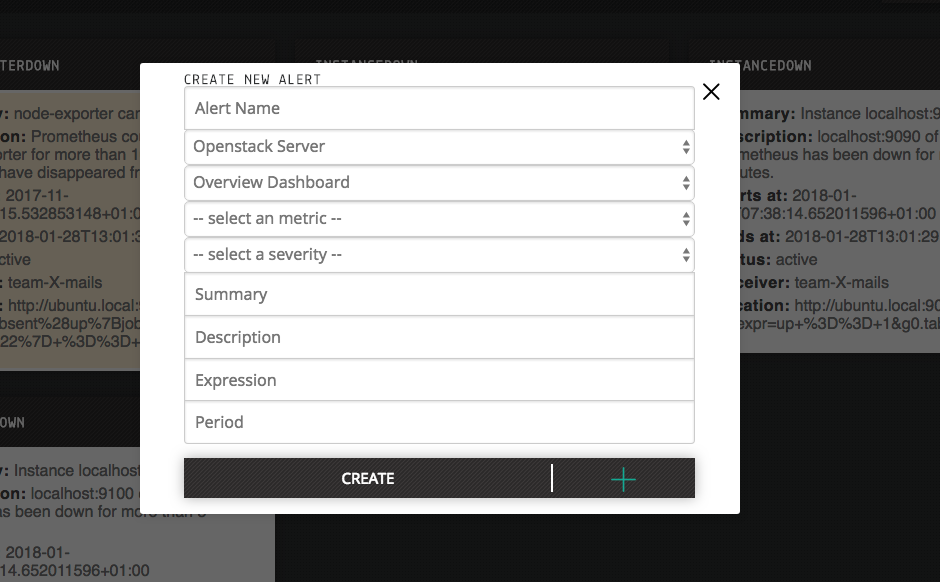
\includegraphics[width=\linewidth]{components/4/pics/alert_create.png}
  \caption{N2Sky Administration Dashboard. Alerting rule creation}
  \label{fig:alert_create}
\end{center}
\end{figure}

The modal window has following elements:
\begin{enumerate}
\item Modal window title is "Create new alert".
\item Combobox with available servers with installed monitoring system.
\item Combobox with a page view, where alert can be shown (optional).
\item Combobox with a available metrics.
\item Combobox wth alerting rule severity level. Three values are possible: "page" for information, "waring" and "critical".
\item Summary information about alerting rule.
\item Full description about alerting rule.
\item Expression which will be executed agains chosen metric.
\item Period, which shows how often will alerting rule validated.
\end{enumerate}

\subsubsection{Alerts representation}\label{Alerts representation}

The alerts are displayed three column grid as it shown in ``Fig.~\ref{fig:alert_representation}'' 

\begin{figure}[htbp]
\begin{center}
  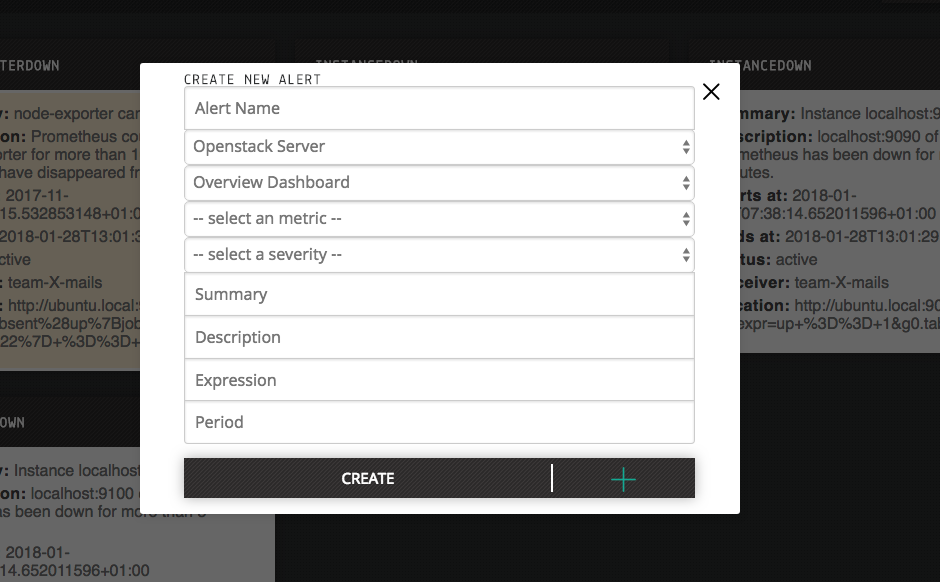
\includegraphics[width=\linewidth]{components/4/pics/alert_create.png}
  \caption{N2Sky Administration Dashboard. Alerts representation}
  \label{fig:alert_representation}
\end{center}
\end{figure}

The view contains:

\begin{description}
\item[Header.] Header is navigation bar  with a title "Fired alerts" and the button. The button has caption "Create Alert" and on click will initiate creating alert rule popup as it described in \autoref{Alerting rule creation} "Alerting rule creation".
\item[Alerts Grid] Contains 3 columns of alerts. When alert end date is earlier then current date, then alert will not be shown. Only active alerts are visible. Detailed information about  alert content is described in \autoref{Alerting Management System} "Alerting Management System".
\end{description}


